% !TEX root = main.tex

\section{运行时系统}
\subsection{存储管理}
\begin{figure}[H]
\centering
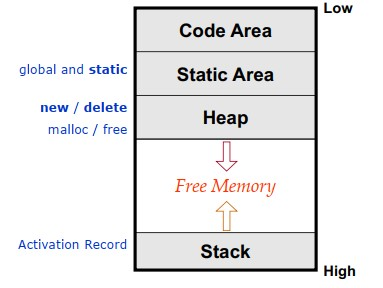
\includegraphics[width=0.5\linewidth]{fig/stack.jpg}
\end{figure}

\subsection{垃圾回收}
\begin{itemize}
	\item 引用计数(reference counting):创建加1,删除减1
	\begin{itemize}
		\item 简单、立即增量式回收
		\item 不能回收循环引用的示例
	\end{itemize}
	\begin{figure}[H]
	\centering
	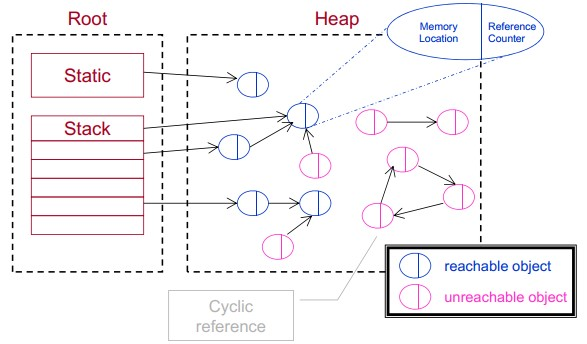
\includegraphics[width=0.8\linewidth]{fig/reference_counting.jpg}
	\end{figure}
	\item 标记扫除(mark and sweep):做图深搜找连通块
	\begin{itemize}
		\item 有办法清除循环引用
		\item 大量垃圾时效率低,无法满足实时应用
	\end{itemize}
	\item 标记压缩(mark and compact):标记,计算新地址,拷贝对象到新地址并更新引用
	\begin{figure}[H]
	\centering
	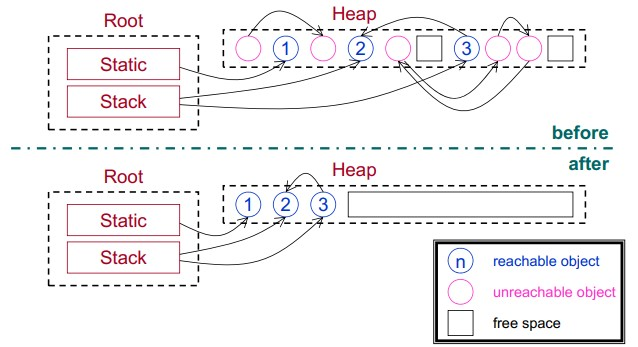
\includegraphics[width=0.8\linewidth]{fig/mark_and_compact.jpg}
	\end{figure}
	\item 拷贝收集(copying collector):堆被划分为两个区域,可达对象一旦被发现就会立即被移动,但不可达对象不做改动
	\begin{figure}[H]
	\centering
	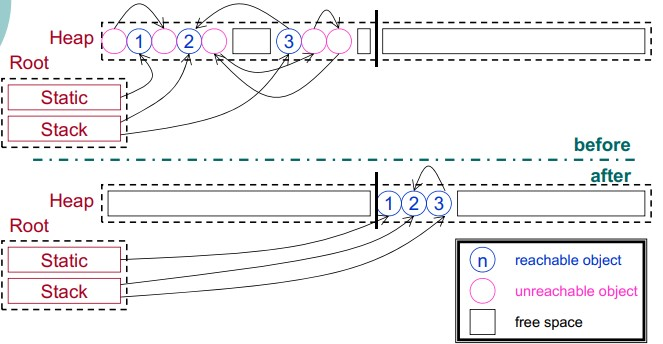
\includegraphics[width=0.8\linewidth]{fig/copying_collector.jpg}
	\end{figure}
\end{itemize}

JVM采用了两代(young \& old)的方式,对于年轻的对象采用拷贝收集,对于老的对象则采用标记压缩。